\documentclass[12pt,a4paper,oneside]{book} % twoside for draf

\usepackage[utf8]{vietnam}
\usepackage[utf8]{inputenc}
\usepackage[unicode]{hyperref}
\usepackage{tipa}
\usepackage{graphicx}
\usepackage{subcaption}
\usepackage{booktabs}
\usepackage{mathptmx}	% same Time New Roma
\usepackage{amsmath}
\usepackage{amssymb}
\usepackage{amsfonts}
\usepackage{sty/ipa}
\usepackage{array}
\newcolumntype{P}[1]{>{\centering\arraybackslash}p{#1}}
\newcolumntype{M}[1]{>{\centering\arraybackslash}m{#1}}
\usepackage{fancyhdr}
\usepackage{multirow}
\usepackage{algorithm2e}
\usepackage{hyperref}
\usepackage{xcolor}
\hypersetup{
    colorlinks=false,
    breaklinks=true,
    citecolor=white,
    citebordercolor=1 1 1,
    filebordercolor=1 1 1,
    linkbordercolor=1 1 1,
    menubordercolor=1 1 1,
    urlbordercolor=1 1 1,
}
\usepackage{xurl}
\usepackage{float}

\usepackage{sty/bkthesis}

\usepackage{graphicx}
\usepackage{listings}
\usepackage{enumitem}

\usepackage{titlesec}
% \titleformat{<command>}[<shape>]{<format>}{<label>}{<sep>}{<before-code>}[<after-code>]
\titleformat{\chapter}[hang]{\normalfont\bfseries}{\thechapter{. }}{0.5em}{\normalfont\bfseries}
\titleformat{\section}[hang]{\normalfont\bfseries}{\thesection{. }}{0.5em}{\normalfont\bfseries}
% \titlespacing*{<command>}{<left>}{<before-sep>}{<after-sep>}
\titlespacing{\chapter}{0pc}{1pc}{0pc}
\titlespacing{\section}{0pc}{0.5pc}{0pc}

\setcounter{secnumdepth}{2}
\crname{Môn học: Học Máy và Ứng Dụng}
\ctname{TÌM HIỂU CÁCH SỬ DỤNG BỘ PHÂN LOẠI CÂY QUYẾT ĐỊNH CỦA THƯ VIỆN SCIKIT-LEARN VÀ ỨNG DỤNG NÓ VÀO BÀI TOÁN PHÂN LOẠI}
\cstuname{
Hồ Phương Ngọc - 1870049
}

\csCouncil{Khoa Khoa Học và Kỹ Thuật Máy Tính}
% \csdeptcode{MÃ NGÀNH: 60.48.01.01}
\csSupervise{GVHD: PGS.TS. Dương Tuấn Anh}
\cttime{ngày 27 tháng 12 năm 2020}

\thesislayout

\begin{document}
%-	Bìa cứng - màu xanh dương
%-	Trang tên (tờ lót): chất liệu giấy, nội dung giống như bìa LV
%-	Mục lục
%-	Danh mục, bảng biểu, hình ảnh, ... (nếu có)
%-	Nội dung LV
%-	Danh mục TL tham khảo
%-	Phụ lục (nếu có)

\coverpage

\frontmatter

\renewcommand*\contentsname{MỤC LỤC}
\tableofcontents
\renewcommand{\listfigurename}{DANH MỤC HÌNH ẢNH}
\listoffigures

\mainmatter

\fancyhead{}  % Clears all page headers and footers
%\rhead{\thepage}  % Sets the right side header to show the page number
%\lhead{}  % Clears the left side page header
%\fancyfoot[positions]{footer}
% \renewcommand{\footrulewidth}{0.4pt}
% \fancyhf{} % sets both header and footer to nothing
\renewcommand{\headrulewidth}{0pt}

\pagestyle{fancy}  % Finally, use the "fancy" page style to implement the FancyHdr headers

\chapter {GIỚI THIỆU}

Bạn có biết rằng, bạn vẫn đang sử dụng phương pháp Cây quyết định (Decision Tree) để đưa ra quyết định trong cả cuộc đời mà không hề hay biết. Hãy xem xét tình huống một người yêu cầu bạn cho họ mượn xe trong một ngày và bạn phải đưa ra quyết định có cho họ mượn xe hay không. Có một số yếu tố giúp xác định quyết định của bạn, một số yếu tố đã được liệt kê bên dưới:

\begin{enumerate}
    \item Người này là bạn thân hay chỉ là người quen? Nếu người đó chỉ là người quen, hãy từ chối yêu cầu; nếu người đó là bạn thì hãy chuyển sang bước tiếp theo.
    \item Người này hỏi mượn xe lần đầu? Nếu vậy, hãy cho họ mượn xe, nếu không thì chuyển sang bước tiếp theo.
    \item Lần trước họ trả xe có bị hư không? Nếu có, hãy từ chối yêu cầu; nếu không, hãy cho họ mượn xe.
\end{enumerate}

Decision Tree cho tình huống nói trên trông giống như sau:

\begin{center}
    \begin{figure}[h!]
        \begin{center}
         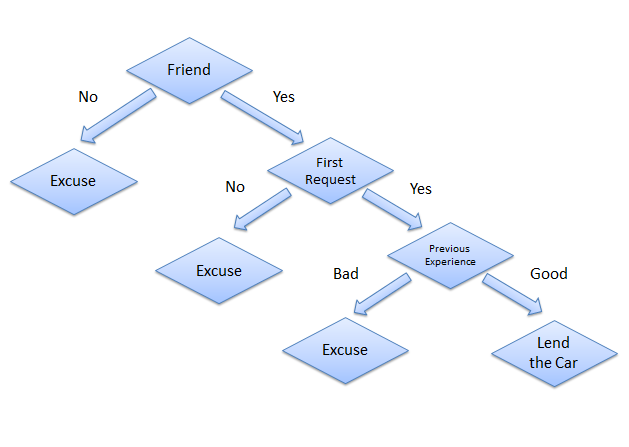
\includegraphics[scale=0.7]{chapter1/img/dt_ex1.png}
        \end{center}
        \caption{Ví dụ về việc ra quyết định dựa trên các câu hỏi.}
        \label{fig:dt_ex1}
    \end{figure}
\end{center}

\begingroup
\renewcommand{\clearpage}{}
\chapter{KHÁI NIỆM CÂY QUYẾT ĐỊNH (DECISION TREE)}

Decision Tree là là một trong những thuật toán supervised learning, được sử dụng thường xuyên và rộng rãi nhất có thể được áp dụng vào cả hai bài toán classification và regression. Việc xây dựng một Decision Tree trên dữ liệu huấn luyện cho trước là việc đi xác định các câu hỏi và thứ tự của chúng. Một điểm đáng lưu ý của Decision Tree là nó có thể làm việc với các đặc trưng (trong các tài liệu về Decision Tree, các đặc trưng thường được gọi là thuộc tính – attribute) dạng categorical, thường là rời rạc và không có thứ tự. Ví dụ, mưa, nắng hay xanh, đỏ, v.v. Decision Tree cũng làm việc với dữ liệu có vector đặc trưng bao gồm cả thuộc tính dạng categorical và liên tục (numeric). Một điểm đáng lưu ý nữa là Decision Tree ít yêu cầu việc chuẩn hoá dữ liệu.


\chapter{THUẬT TOÁN CÂY QUYẾT ĐỊNH (DECISION TREE)}

Decision Tree có nhiều thuật toán khác nhau.

\begin{itemize}
    \item ID3:\\
    ID3 (Iterative Dichotomiser 3) được phát triển vào nào 1986 bởi Ross Quinlan. Sử dụng lượng thông tin ứng với biến số phân loại sau đó dùng kỹ thuật tham lam (lựa chọn tối ưu địa phương ở mỗi bước đi với hy vọng tìm được tối ưu toàn cục).\\
    Ví dụ như thuật toán tìm đường đi ngắn nhất của Dijkstra.
    \item C4.5:\\
    Được phát triển từ ID3. C4.5 là thuật toán phân lớp dữ liệu dựa trên cây quyết định hiệu quả và phổ biến trong những ứng dụng khai phá cơ sở dữ liệu có kích thước nhỏ.\\
    So với ID3, C4.5 không cần biến số phân loại lượng đặc trưng. Output theo dạng if-then, không hiển thị những phần cành không cần thiết.
    \item C5.0:\\
    Là bản cải tiến của C4.5. Giúp cải thiện vấn đề hiệu năng và sử dụng ít bộ nhớ hơn.
    \item CART:\\
    CART (Classification and Regression Trees) khá giống với C4.5. Được phát triển bởi Breiman năm 1984. Tạo cây phân tích dựa trên biến phân loại, giải thích, mục đính và hồi quy.
\end{itemize}

\chapter{CÔNG THỨC TOÁN HỌC}

\section{Entropy}
Entropy là thuật ngữ thuộc Nhiệt động lực học, là thước đo của sự biến đổi, hỗn loạn hoặc ngẫu nhiên. Năm 1948, Shannon đã mở rộng khái niệm Entropy sang lĩnh vực nghiên cứu, thống kê với công thức như sau:\\

Với một phân phối xác suất của một biến rời rạc $x$ có thể nhận $n$ giá trị khác nhau $x_1, x_2,..., x_n$\\

Giả sử rằng xác suất để $x$ nhận các giá trị này là $p_i=p(x=x_i)$.\\

Ký hiệu phân phối này là $p=(p_1, p_2,..., p_n)$. Entropy của phân phối này được định nghĩa là:

\begin{equation*}
    H(p)=-\sum_{n=1}^{n}p_ilog(p_i)
\end{equation*}

trong đó $log$ là logarit tự nhiên (Một số tài liệu dùng logarit cơ số 2, nhưng giá trị của $H(p)$ chỉ khác đi bằng cách nhân với một hằng số.) và quy ước $0log(0)=0$\\

Giả sử bạn tung một đồng xu, Entropy sẽ được tính như sau:

\begin{equation*}
    H = -[0.5log(0.5) + 0.5log(0.5)]
\end{equation*}

\begin{center}
    \begin{figure}[ht!]
        \begin{center}
         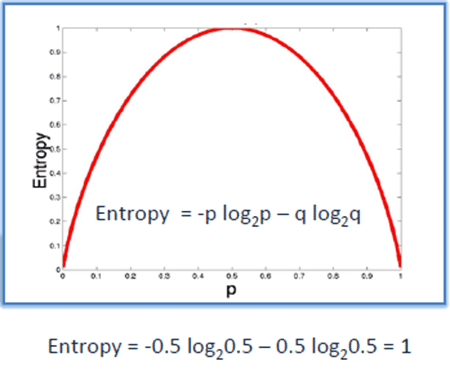
\includegraphics[scale=0.7]{chapter4/img/dt_ex2.png}
        \end{center}
        \caption{Hàm Entropy.}
        \label{fig:dt_ex2}
    \end{figure}
\end{center}

Hình vẽ trên biểu diễn sự thay đổi của hàm Entropy. Ta có thể thấy rằng, Entropy đạt tối đa khi xác suất xảy ra của hai lớp bằng nhau.

\begin{itemize}
    \item P tinh khiết: $p_i=0$ hoặc $p_i=1$
    \item P vẩn đục: $p_i=0.5$, khi đó hàm Entropy đạt đỉnh cao nhất
\end{itemize}

Entropy trong học máy và lý thuyết thông tin nói chung là thước đo tính ngẫu nhiên của thông tin đang được xử lý. Entropy càng cao, càng khó rút ra bất kỳ kết luận nào từ thông tin đó. Tung một đồng xu là một ví dụ về thông tin ngẫu nhiên, trong trường hợp này Entropy đạt cực đại bằng 1, không có kết luận nào giúp dự đoán được kết quả tung đồng xu.

\section{Information Gain}
Information Gain dựa trên sự giảm của hàm Entropy khi tập dữ liệu được phân chia trên một thuộc tính. Để xây dựng một Decision Tree, ta phải tìm tất cả thuộc tính trả về Infomation Gain cao nhất.

Để xác định các nút trong mô hình Decision Tree, ta thực hiện tính Infomation Gain tại mỗi nút theo trình tự sau:

\begin{itemize}
    \item \textbf{Bước 1:} Tính toán hệ số Entropy của biến mục tiêu $S$ có $N$ phần tử với $N_c$ phần tử thuộc lớp $c$ cho trước:
    \begin{equation*}
        H(S) = -\sum_{c=1}^{c}(N_c/N)log(N_c/N)
    \end{equation*}
    
    \item \textbf{Bước 2:} Tính hàm số Entropy tại mỗi thuộc tính: với thuộc tính $x$, các điểm dữ liệu trong $S$ được chia ra $K$ child node $S_1, S_2,..., S_K$ với số điểm trong mỗi child node lần lượt là $m_1, m_2,..., m_K$, ta có:
    \begin{equation*}
        H(x, S) = \sum_{K=1}^{K}(m_K/N)*H(S_K)
    \end{equation*}
    
    \item \textbf{Bước 3:} Chỉ số Gain Information được tính bằng:
    \begin{equation*}
        G(x, S) = H(S) - H(x, S)
    \end{equation*}
\end{itemize}

\section{Gini Impurity}
Đơn giản hơn so với Entropy và Information Gain, Gini Impurity là chỉ số thể hiện mức độ phân loại sai khi ta chọn ngẫu nhiên một phần tử từ tập data. Gini Impurity có công thức như sau:

\begin{equation*}
    G = \sum_{k=1}^{k}p_k*(1-p_k)^2 = 1 - \sum_{k=1}^{k}(p_k)^2
\end{equation*}

Trong đó:
\begin{itemize}
    \item $G$ là giá trị Gini Impurity
    \item $k$ số các lớp có trong tập data
    \item $p_k$ là xác suất mà một phần tử ngẫu nhiên thuộc lớp $k$
\end{itemize}

Giá trị Gini Impurity sau khi chia của mỗi nhóm đều nhỏ hơn so với giá trị ban đầu => Sau khi chia nhóm mức độ phân loại sai của hệ thống đã giảm. Độ giảm của Gini Impurity được gọi là Gini Gain và có công thức tính tương tự như Information Gain, chỉ khác là ta sẽ sử dụng giá trị Gini Impurity thay vì Entropy:

\begin{equation*}
    GG(Q) = G_O - \sum_{i=1}^{q}\frac{N_i}{N}G_i
\end{equation*}

Cũng tương tự như với khi sử dụng Entropy, Gini Impurity của một Leaf Node sẽ là 0 và khi training Decision Tree, điều kiện được chọn để chia nhóm cũng sẽ được chọn sao cho giá trị Gini Gain là lớn nhất.


\chapter{ƯU NHƯỢC ĐIỂM CỦA CÂY QUYẾT ĐỊNH (DECISION TREE)}

\section{Một số ưu điểm của Decision Tree}
Cây quyết định là một thuật toán đơn giản và phổ biến. Thuật toán này được sử dụng rộng rãi bới những lợi ích của nó:

\begin{itemize}
    \item Mô hình sinh ra các quy tắc dễ hiểu cho người đọc, tạo ra bộ luật với mỗi nhánh lá là một luật của cây.
    \item Việc chuẩn bị dữ liệu cho một Decision Tree là cơ bản hoặc không cần thiết. Các kỹ thuật khác thường đòi hỏi chuẩn hóa dữ liệu, cần tạo các biến phụ (dummy variable) và loại bỏ các giá trị rỗng.
    \item Cây quyết định có thể xử lý cả dữ liệu có giá trị bằng số và dữ liệu có giá trị là tên thể loại. Tuy nhiên, hiện tại việc triển khai trong scikit-learn không hỗ trợ các biến phân loại. Các kỹ thuật khác thường chuyên để phân tích các bộ dữ liệu chỉ gồm một loại biến. Chẳng hạn, các luật quan hệ chỉ có thể dùng cho các biến tên, trong khi mạng nơ-ron chỉ có thể dùng cho các biến có giá trị bằng số.
    \item Cây quyết định là một mô hình hộp trắng. Nếu có thể quan sát một tình huống cho trước trong một mô hình, thì có thể dễ dàng giải thích điều kiện đó bằng logic Boolean. Mạng nơ-ron là một ví dụ về mô hình hộp đen, do lời giải thích cho kết quả quá phức tạp để có thể hiểu được.
    \item Có thể thẩm định một mô hình bằng các kiểm tra thống kê. Điều này làm cho ta có thể tin tưởng vào mô hình.
    \item Cây quyết định có thể xử lý tốt một lượng dữ liệu lớn trong thời gian ngắn. Có thể dùng máy tính cá nhân để phân tích các lượng dữ liệu lớn trong một thời gian đủ ngắn để cho phép các nhà chiến lược đưa ra quyết định dựa trên phân tích của Decision Tree.
    \item Chi phí sử dụng cây (tức là dữ liệu dự đoán) được tính theo lôgarit trong số điểm dữ liệu được sử dụng để đào tạo cây.
    \item Có khả năng xử lý các vấn đề đa đầu ra.
\end{itemize}

\section{Một số nhược điểm của Decision Tree}
Kèm với đó, Decision Tree cũng có những nhược điểm cụ thể:

\begin{itemize}
    \item Mô hình Decision Tree phụ thuộc rất lớn vào dữ liệu của bạn. Thậm chí, với một sự thay đổi nhỏ trong bộ dữ liệu, cấu trúc mô hình Decision Tree có thể thay đổi hoàn toàn.
    \item Decision Tree hay gặp vấn đề overfitting.
    \item Khó giải quyết được những vấn đề có dữ liệu phụ thuộc thời gian liên tục.
    \item Dễ xảy ra lỗi khi có quá nhiều lớp chi phí tính toán để xây dựng mô hình Decision Tree cao.
\end{itemize}

\chapter{THƯ VIỆN SCIKIT-LEARN}

\section{Sự hình thành}
Scikit-learn ban đầu được đề xuất bởi David Cournapeau trong một dự án mùa hè của Google vào năm 2007.\\

Later Matthieu Brucher tham gia dự án trên và bắt đầu sử dụng nó làm một phần luận văn tiến sĩ của ông ấy. Vào năm 2010, INRIA bắt đầu tài trợ và phiên bản đầu tiên được xuất bản (v0.1 beta) vào cuối tháng 1 năm 2010.\\

Dự án vẫn đang được nghiên cứu bởi một đội ngũ hơn 30 nhà nghiên cứu đến từ các công ty lớn INRIA, Google, Tinyclues và Python Software Foundation.

\section{Scikit-learn là gì?}
Scikit-learn (Sklearn) là thư viện mạnh mẽ nhất dành cho các thuật toán học máy được viết trên ngôn ngữ Python. Thư viện cung cấp một tập các công cụ xử lý các bài toán machine learning và statistical modeling gồm: classification, regression, clustering, và dimensionality reduction.\\

Thư viện được cấp phép bản quyền chuẩn FreeBSD và chạy được trên nhiều nền tảng Linux. Scikit-learn được sử dụng như một tài liệu để học tập.\\

Để cài đặt scikit-learn trước tiên phải cài thư viện SciPy (Scientific Python). Những thành phần gồm:

\begin{itemize}
    \item \textbf{Numpy:} Gói thư viện xử lý dãy số và ma trận nhiều chiều.
    \item \textbf{SciPy:} Gói các hàm tính toán logic khoa học.
    \item \textbf{Matplotlib:} Biểu diễn dữ liệu dưới dạng đồ thị 2 chiều, 3 chiều.
    \item \textbf{IPython:} Notebook dùng để tương tác trực quan với Python.
    \item \textbf{SymPy:} Gói thư viện các kí tự toán học.
    \item \textbf{Pandas:} Xử lý, phân tích dữ liệu dưới dạng bảng.
\end{itemize}

Những thư viện mở rộng của SciPy thường được đặt tên dạng SciKits. Như thư viện này là gói các lớp, hàm sử dụng trong thuật toán học máy thì được đặt tên là scikit-learn.\\

Scikit-learn hỗ trợ mạnh mẽ trong việc xây dựng các sản phẩm. Nghĩa là thư viện này tập trung sâu trong việc xây dựng các yếu tố: dễ sử dụng, dễ code, dễ tham khảo, dễ làm việc, hiệu quả cao.\\

Mặc dù được viết cho Python nhưng thực ra các thư viện nền tảng của scikit-learn lại được viết dưới các thư viện của C để tăng hiệu suất làm việc. Ví dụ như: Numpy(Tính toán ma trận), LAPACK, LibSVM và Cython.


\chapter{ỨNG DỤNG CÂY QUYẾT ĐỊNH (DECISION TREE) CHO BÀI TOÁN PHÂN LOẠI VỚI SCIKIT-LEARN}

\section{Tập dữ liệu hoa Iris (Iris flower dataset)}
Iris flower dataset là một bộ dữ liệu nhỏ. Bộ dữ liệu này bao gồm thông tin của ba loại hoa Iris (một loài hoa lan) khác nhau: Iris setosa, Iris virginica và Iris versicolor. Mỗi loại có 50 bông hoa được đo với dữ liệu là 4 thông tin: chiều dài, chiều rộng đài hoa (sepal), và chiều dài, chiều rộng cánh hoa (petal). Dưới đây hình \ref{fig:iris} là ví dụ về hình ảnh của ba loại hoa.\newpage

\begin{center}
    \begin{figure}[h!]
        \begin{center}
         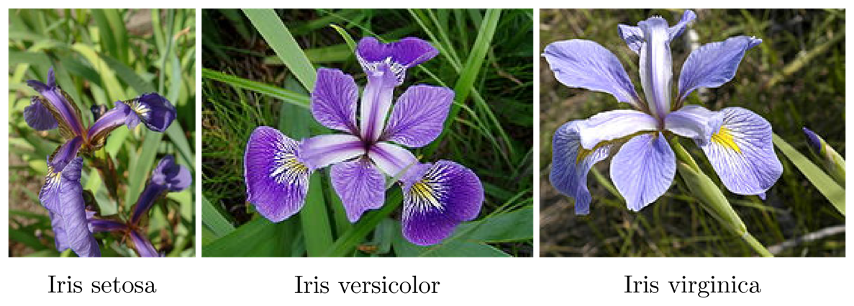
\includegraphics[scale=0.7]{chapter7/img/iris.png}
        \end{center}
        \caption{Ví dụ về Iris flower dataset}
        \label{fig:iris}
    \end{figure}
\end{center}

Bộ dữ liệu nhỏ này thường được sử dụng trong nhiều thuật toán Machine Learning trong các lớp học.

\section{Xây dựng mô hình}
\textbf{Import thư viện và tập dữ liệu:}

Trước tiên, chúng ta cần khai báo vài thư viện và load dữ liệu Iris flower dataset.

Vì tệp ở định dạng CSV, nên sử dụng phương thức read\_csv của panda để đọc tệp dữ liệu CSV.

\begin{center}
\begin{lstlisting}[language=Python,breaklines=true]
import pandas as pd
import numpy as np
# load data
dataset = pd.read_csv('Iris.csv')
\end{lstlisting}
\end{center}

\textbf{Phân tích dữ liệu:}

Thực thi lệnh sau để xem số hàng và cột trong tập dữ liệu.

\begin{center}
\begin{lstlisting}[language=Python,breaklines=true]
# get how many instances (rows) and how many attributes (columns)
dataset.shape
\end{lstlisting}
\end{center}

Kết quả đầu ra sẽ hiển thị "(150, 6)", có nghĩa là tập dữ liệu có 150 bản ghi và 6 thuộc tính.\\

Thực thi lệnh sau để xem các thông tin cơ bản: giá trị cột dữ liệu lớn nhất, nhỏ nhất, và trung bình.

\begin{center}
\begin{lstlisting}[language=Python,breaklines=true]
# show basic info: max, min, mean of dataset columns
dataset.describe()
\end{lstlisting}
\end{center}

Kết quả đầu ra như bảng dưới.

\begin{center}
\begin{lstlisting}[basicstyle=\fontsize{10}{13}\selectfont\ttfamily]
      Id         SepalLengthCm SepalWidthCm PetalLengthCm PetalWidthCm
count 150.000000 150.000000    150.000000   150.000000    150.000000
mean  75.500000  5.843333      3.054000     3.758667      1.198667
std   43.445368  0.828066      0.433594     1.764420      0.763161
min   1.000000   4.300000      2.000000     1.000000      0.100000
25%   38.250000  5.100000      2.800000     1.600000      0.300000
50%   75.500000  5.800000      3.000000     4.350000      1.300000
75%   112.750000 6.400000      3.300000     5.100000      1.800000
max   150.000000 7.900000      4.400000     6.900000      2.500000
\end{lstlisting}
\end{center}

Thực thi lệnh sau để xem dữ liệu thống kê của các cột (bao gồm các cột phân loại).

\begin{center}
\begin{lstlisting}[language=Python,breaklines=true]
# display statistical data of columns (including categorical columns)
dataset.describe(include = 'all')
\end{lstlisting}
\end{center}

Kết quả đầu ra như bảng dưới.

\begin{center}
\begin{lstlisting}[basicstyle=\fontsize{8.5}{13}\selectfont\ttfamily]
       Id         SepalLengthCm SepalWidthCm PetalLengthCm PetalWidthCm Species
count  150.000000 150.000000    150.000000   150.000000    150.000000   150
unique NaN        NaN           NaN          NaN           NaN          3
top    NaN        NaN           NaN          NaN           NaN          Iris-setosa
freq   NaN        NaN           NaN          NaN           NaN          50
mean   75.500000  5.843333      3.054000     3.758667      1.198667     NaN
std    43.445368  0.828066      0.433594     1.764420      0.763161     NaN
min    1.000000   4.300000      2.000000     1.000000      0.100000     NaN
25%    38.250000  5.100000      2.800000     1.600000      0.300000     NaN
50%    75.500000  5.800000      3.000000     4.350000      1.300000     NaN
75%    112.750000 6.400000      3.300000     5.100000      1.800000     NaN
max    150.000000 7.900000      4.400000     6.900000      2.500000     NaN
\end{lstlisting}
\end{center}

Thực thi lệnh sau để kiểm tra năm bản ghi đầu tiên của tập dữ liệu.

\begin{center}
\begin{lstlisting}[language=Python,breaklines=true]
# show some first rows
dataset.head(5)
\end{lstlisting}
\end{center}

Kết quả đầu ra như bảng dưới.

\begin{center}
\begin{lstlisting}[basicstyle=\fontsize{10}{13}\selectfont\ttfamily]
  Id SepalLengthCm SepalWidthCm PetalLengthCm PetalWidthCm Species
0 1  5.1           3.5          1.4           0.2          Iris-setosa
1 2  4.9           3.0          1.4           0.2          Iris-setosa
2 3  4.7           3.2          1.3           0.2          Iris-setosa
3 4  4.6           3.1          1.5           0.2          Iris-setosa
4 5  5.0           3.6          1.4           0.2          Iris-setosa
\end{lstlisting}
\end{center}

Thực thi lệnh sau để kiểm tra năm bản ghi cuối của tập dữ liệu.

\begin{center}
\begin{lstlisting}[language=Python,breaklines=true]
# show some last rows
dataset.tail(5)
\end{lstlisting}
\end{center}

Kết quả đầu ra như bảng dưới.

\begin{center}
\begin{lstlisting}[basicstyle=\fontsize{9}{13}\selectfont\ttfamily]
    Id  SepalLengthCm SepalWidthCm PetalLengthCm PetalWidthCm Species
145 146 6.7           3.0          5.2           2.3          Iris-virginica
146 147 6.3           2.5          5.0           1.9          Iris-virginica
147 148 6.5           3.0          5.2           2.0          Iris-virginica
148 149 6.2           3.4          5.4           2.3          Iris-virginica
149 150 5.9           3.0          5.1           1.8          Iris-virginica
\end{lstlisting}
\end{center}

Thực thi lệnh sau để xem số lượng instance (hàng) thuộc về từng lớp.

\begin{center}
\begin{lstlisting}[language=Python,breaklines=true]
# numbers of instances (rows) that belong to each class. 
dataset.groupby('Species').size()
\end{lstlisting}
\end{center}

Kết quả đầu ra như bảng dưới. Thấy được, mỗi loại hoa đều có 50 mẫu.

\begin{center}
\begin{lstlisting}[language=Python,breaklines=true]
Species
Iris-setosa        50
Iris-versicolor    50
Iris-virginica     50
dtype: int64
\end{lstlisting}
\end{center}

\textbf{Tiền xử lý dữ liệu:}

Trong phần này, tôi chia dữ liệu của mình thành các thuộc tính và nhãn và sau đó sẽ chia dữ liệu kết quả thành cả tập huấn luyện và tập kiểm tra. Bằng cách này, chúng tôi có thể huấn luyện thuật toán của mình trên một tập dữ liệu và sau đó kiểm tra nó trên một tập dữ liệu hoàn toàn khác mà thuật toán chưa thấy. Điều này cung cấp cho chúng ta cái nhìn chính xác hơn về cách thuật toán được đào tạo sẽ thực sự hoạt động.\\

Để chia dữ liệu thành các thuộc tính và nhãn, thực thi đoạn mã sau.

\begin{center}
\begin{lstlisting}[language=Python,breaklines=true]
feature_columns = ['SepalLengthCm', 'SepalWidthCm', 'PetalLengthCm','PetalWidthCm']
X = dataset[feature_columns].values
y = dataset['Species'].values
\end{lstlisting}
\end{center}

Ở đây biến $X$ chứa tất cả các cột từ tập dữ liệu, ngoại trừ cột "Species", là nhãn. Biến $y$ chứa các giá trị từ cột "Species". Biến $X$ là tập thuộc tính của chúng ta và biến $y$ chứa các nhãn tương ứng.\\

Bước tiền xử lý cuối cùng là chia dữ liệu thành các tập huấn luyện và thử nghiệm. Thư viện model\_selection của scikit-learn chứa phương thức train\_test\_split, chúng tôi sẽ sử dụng phương thức này để chia ngẫu nhiên dữ liệu thành các tập huấn luyện và thử nghiệm.

\begin{center}
\begin{lstlisting}[language=Python,breaklines=true]
from sklearn.model_selection import train_test_split
X_train, X_test, y_train, y_test = train_test_split(X, y, test_size = 0.3, random_state = 0)
\end{lstlisting}
\end{center}

Trong đoạn mã trên, tham số test\_size chỉ định tỷ lệ của tập thử nghiệm, ở đây sử dụng 30\% dữ liệu cho tập thử nghiệm và 70\% cho tập huấn luyện.\\

\textbf{Đào tạo và đưa ra dự đoán:}

Khi dữ liệu đã được chia thành các tập huấn luyện và thử nghiệm, bước cuối cùng là huấn luyện thuật toán Decision Tree trên dữ liệu này và đưa ra dự đoán. Scikit-learn chứa các class/phương thức tích hợp sẵn cho các thuật toán Decision Tree khác nhau. Để sử dụng cho bài toán phân loại, sử dụng class $DecisionTreeClassifier$. Phương thức $fit$ của class này được gọi để huấn luyện thuật toán trên dữ liệu huấn luyện, được truyền dưới dạng tham số cho phương thức $fit$. Ngoài ra, ở đây ta sử dụng hai độ đo khác nhau, là "Gini" và "Entropy", tạo ra hai mô hình khác nhau.

\begin{enumerate}[label=(\alph*)]
    \item \textbf{criterion='gini'}
    
    Thực thi tập lệnh sau để huấn luyện thuật toán.
    
    \begin{center}
    \begin{lstlisting}[language=Python,breaklines=true]
    from sklearn.tree import DecisionTreeClassifier  
    dt = DecisionTreeClassifier(criterion='gini')  
    dt.fit(X_train, y_train)
    \end{lstlisting}
    \end{center}

    Bây giờ bộ phân loại đã được đào tạo, hãy đưa ra dự đoán trên dữ liệu thử nghiệm. Để đưa ra dự đoán, phương pháp dự đoán của lớp DecisionTreeClassifier được sử dụng. Hãy xem đoạn mã sau để sử dụng.
    
    \begin{center}
    \begin{lstlisting}[language=Python,breaklines=true]
    y_pred_dt = dt.predict(X_test)
    \end{lstlisting}
    \end{center}

    \textbf{Đánh giá thuật toán:}
    
    Tại thời điểm này, tôi đã đào tạo thuật toán của mình và đưa ra một số dự đoán. Bây giờ chúng ta sẽ xem thuật toán của chúng ta chính xác đến mức nào. Đối với các nhiệm vụ phân loại, một số chỉ số thường được sử dụng là ma trận nhầm lẫn, độ chính xác, thu hồi và điểm F1. Thư viện của scikit-learn chứa phương thức classification\_report và confusion\_matrix có thể được sử dụng để tính toán các số liệu này.
    
    \begin{center}
    \begin{lstlisting}[language=Python,breaklines=true]
    from sklearn.metrics import classification_report, confusion_matrix
    print(confusion_matrix(y_test, y_pred_dt))
    print(classification_report(y_test, y_pred_dt))
    dt_score = dt.score(X_test, y_test)
    print(f"Decision Tree classifier accuracy score is %.2f" % dt_score)
    \end{lstlisting}
    \end{center}

    Kết quả như bên dưới.
    
    \begin{center}
    \begin{lstlisting}[basicstyle=\fontsize{11}{13}\selectfont\ttfamily]
    [[16  0  0]
     [ 0 17  1]
     [ 0  0 11]]
                     precision    recall  f1-score   support
    
        Iris-setosa       1.00      1.00      1.00        16
    Iris-versicolor       1.00      0.94      0.97        18
     Iris-virginica       0.92      1.00      0.96        11
    
           accuracy                           0.98        45
          macro avg       0.97      0.98      0.98        45
       weighted avg       0.98      0.98      0.98        45
    
    Decision Tree classifier accuracy score is 0.98
    \end{lstlisting}
    \end{center}

    Từ confusion\_matrix, có thể thấy rằng trong số 45 trường hợp thử nghiệm, thuật toán chỉ phân loại sai 1. Đây là độ chính xác 98\%.
    
    \item \textbf{criterion='entropy'}
    
    Thực thi tập lệnh sau để huấn luyện thuật toán.
    
    \begin{center}
    \begin{lstlisting}[language=Python,breaklines=true]
    from sklearn.tree import DecisionTreeClassifier  
    dt = DecisionTreeClassifier(criterion='entropy')  
    dt.fit(X_train, y_train)
    \end{lstlisting}
    \end{center}

    Dự đoán trên dữ liệu thử nghiệm.
    
    \begin{center}
    \begin{lstlisting}[language=Python,breaklines=true]
    y_pred_dt = dt.predict(X_test)
    \end{lstlisting}
    \end{center}

    \textbf{Đánh giá thuật toán:}
    
    \begin{center}
    \begin{lstlisting}[language=Python,breaklines=true]
    from sklearn.metrics import classification_report, confusion_matrix
    print(confusion_matrix(y_test, y_pred_dt))
    print(classification_report(y_test, y_pred_dt))
    dt_score = dt.score(X_test, y_test)
    print(f"Decision Tree classifier accuracy score is %.2f" % dt_score)
    \end{lstlisting}
    \end{center}

    Kết quả như bên dưới.
    
    \begin{center}
    \begin{lstlisting}[basicstyle=\fontsize{11}{13}\selectfont\ttfamily]
    [[16  0  0]
     [ 0 17  1]
     [ 0  0 11]]
                     precision    recall  f1-score   support
    
        Iris-setosa       1.00      1.00      1.00        16
    Iris-versicolor       1.00      0.94      0.97        18
     Iris-virginica       0.92      1.00      0.96        11
    
           accuracy                           0.98        45
          macro avg       0.97      0.98      0.98        45
       weighted avg       0.98      0.98      0.98        45
    
    Decision Tree classifier accuracy score is 0.98
    \end{lstlisting}
    \end{center}

    Kết quả không khác gì so với sử dụng độ đo "Gini".
\end{enumerate}


% \input{chapter8/chapter8.tex}
\endgroup

\titlespacing{\chapter}{0pc}{1pc}{1pc}
%bibliography{refs}{}
%bibliographystyle{plain}
%-	Danh mục TL tham khảo
%-	Phụ lục (nếu có)
\renewcommand\bibname{TÀI LIỆU THAM KHẢO}

\begin{thebibliography}{}

% reference in chapter 1
\bibitem{decisiontreesinpythonwithscikitlearn} 
Scott Robinson, Decision Trees in Python with Scikit-Learn
\\\url{https://stackabuse.com/decision-trees-in-python-with-scikit-learn/}

% reference in chapter 3
\bibitem{userguide}
Scikit-learn, User Guide
\\\url{https://scikit-learn.org/stable/modules/tree.html#}

% reference in chapter 6
\bibitem{scikitlearn}
Thư Viện Scikit-learn Trong Python Là Gì?
\\\url{https://codelearn.io/sharing/scikit-learn-trong-python-la-gi}

% reference in chapter 7
\bibitem{decisiontreeclassifier}
Scikit-learn, class sklearn.tree.DecisionTreeClassifier
\\\url{https://scikit-learn.org/stable/modules/generated/sklearn.tree.DecisionTreeClassifier.html}

\end{thebibliography}

\end{document}